% Straight up stealing preamble from Eli Holmes 
%%%%%%%%%%%%%%%%%%%%%%%%%%%%%%%%%%%%%%START PREAMBLE THAT IS THE SAME FOR ALL EXAMPLES
\documentclass{article}

%Required: You must have these
\usepackage{Sweave}
\usepackage{graphicx}
\usepackage{tabularx}
\usepackage{hyperref}
\usepackage{natbib}
\usepackage{pdflscape}
\usepackage{array}
\usepackage{authblk}
\usepackage{gensymb}


%\usepackage[backend=bibtex]{biblatex}
%Strongly recommended
  %put your figures in one place
%\SweaveOpts{prefix.string=figures/, eps=FALSE} 
%you'll want these for pretty captioning
\usepackage[small]{caption}

\setkeys{Gin}{width=0.8\textwidth}  %make the figs 50 perc textwidth
\setlength{\captionmargin}{30pt}
\setlength{\abovecaptionskip}{10pt}
\setlength{\belowcaptionskip}{10pt}
% manual for caption  http://www.dd.chalmers.se/latex/Docs/PDF/caption.pdf

%Optional: I like to muck with my margins and spacing in ways that LaTeX frowns on
%Here's how to do that
\topmargin -1.5cm        
\oddsidemargin -0.04cm   
\evensidemargin -0.04cm  % same as oddsidemargin but for left-hand pages
\textwidth 16.59cm
\textheight 21.94cm 
%\pagestyle{empty}       % Uncomment if don't want page numbers
\parskip 7.2pt           % sets spacing between paragraphs
%\renewcommand{\baselinestretch}{1.5} 	% Uncomment for 1.5 spacing between lines
\parindent 0pt% sets leading space for paragraphs
\usepackage{setspace}
%\doublespacing

%Optional: I like fancy headers
%\usepackage{fancyhdr}
%\pagestyle{fancy}
%\fancyhead[LO]{How do climate change experiments actually change climate}
%\fancyhead[RO]{2016}
 
%%%%%%%%%%%%%%%%%%%%%%%%%%%%%%%%%%%%%%END PREAMBLE THAT IS THE SAME FOR ALL EXAMPLES

%Start of the document
\begin{document}


%\SweaveOpts{concordance=TRUE}

\bibliographystyle{..//..//refs/bibstyles/amnat.bst}
\title{Spatial and temporal shifts in photoperiod with climate change} % perspective paper for OSPREE analyses


\author[1,2,a]{A. K. Ettinger}
\author[2,3]{D. M. Buonaiuto}

\author[2,3]{C. J. Chamberlain}

\author[2,3,4,5]{I. Morales-Castilla}

\author[2,3,6]{E. M. Wolkovich}

\affil[1]{Northwest Fisheries Science Center, NOAA, Seattle, Washington, USA}

\affil[2]{Arnold Arboretum of Harvard University, Boston, Massachusetts, USA}


\affil[3]{Department of Organismic and Evolutionary Biology, Harvard University, Cambridge, Massachusetts, USA}

\affil[4]{Department of Life Sciences, University of Alcal\`a CTRA N-II, KM., 33,600, 28802, Alcal\`a de Henares, Spain}

\affil[5]{Department of Environmental Science and Policy, George Mason  University, Fairfax, Virginia, USA}
 
\affil[6]{Forest \& Conservation Sciences, Faculty of Forestry, University of British Columbia, Vancouver, British Columbia, Canada}

\affil[a]{Corresponding author; email: ailene.ettinger@noaa.gov; phone: 781-296-4821; mailing address: Northwest Fisheries Science Center, NOAA, 2725 Montlake Blvd W, Seattle, WA 98118 USA}

\date{} 

\maketitle %put the fancy title on

\textbf{Data Accessibility} The OSPREE database is available at KNB, doi:10.5063/F1QV3JQR \citep{wolkovich2019}.

\textbf{Running head} Shifts in photoperiod with climate change

\textbf{Key words} phenology, global warming, range shifts, timing, spring, budburst,daylength 

\textbf{Paper type} Opinion

%\tableofcontents      %add a table of contents
%\clearpage
%New goal is GCB Perspective
%In lieu of a cover letter, authors must answer the following questions during submission (max 50 words per answer):

%    What is the scientific question you are addressing?
%    What is/are the key finding(s) that answers this question?
%    Why is this work important and timely?
%    Does your paper fall within the scope of GCB; what biological AND global change aspects does it address?
%    What are the three most recently published papers that are relevant to this question? This information will assist the Editors in selecting reviewers.

%Opinion articles should be no more than 5000 words and have no more than 8 tables and figures. 
%%%%%%%%%%%%%%%%%%%%%%%%%%%%%%%%%%%%%%%%%%%%%%%%%%%

%%%%%%%%%%%%%%%%%%%%%%%%%%%%%%%%%%%%%%%%%%%%%%%%%%%

\section*{Abstract}
Climate change causes both temporal and geographic shifts in species; these shifts in turn affect the daylength (photoperiod) that species experience. As photoperiod is a common trigger of seasonal biological responses (e.g., affecting plant phenology in 84\% of studies that manipulated photoperiod), such shifts in experienced photoperiod may have important implications for future distributions and fitness of many species. However, photoperiod has not been a focus of climate change forecasting to date, especially for early-season (`spring') events---which are often assumed to be driven by temperature. Here we show that impacts on experienced photoperiod due to temporal shifts could be quite large and may be orders of magnitude larger than impacts due to spatial shifts (e.g., 1.6 hours of change for expected temporal shifts versus only one minute for spatial shifts). Incorporating these effects into forecasts may be possible by leveraging existing experimental data; for example, growth chamber experiments on woody plant spring phenology often have data relevant for climate change impacts. We highlight how combining novel modeling approaches and empirical work on when, where, and how much photoperiod affects spring phenology, could rapidly advance our understanding and predictions of future spatial-temporal shifts due to climate change. %currently 197 words 


\section*{Introduction}
\par Shifts in the timing of spring events---i.e., phenology, including flowering, bird arrival, egg hatching and myriad other biological activities---are some of the most widely documented signals of climate change. Across taxa, from plants and insects to mollusks and mammals, spring phenology is occurring earlier as temperatures warm, with average shifts of 1.2 to 5.1 days earlier per decade \citep{bradley1999,parmesan2003, poloczanska2013,root2003} or 1.3 to 5.6 days earlier per \degree C of warming \citep{polgar2013,Wolkovich:2012n}. These changes are some of the largest climate change induced shifts observed, with early spring phenology shifting more rapidly than later season phenology in most cases \citep{bradley1999,menzel2006}, and suggest that temperature is a major driver of spring phenophases.

\par Spring phenology is not controlled solely by temperature, however. Photoperiod is also a critical cue for plants and animals, signaling changes in growth, mating, and reproduction across diverse species \citep[e.g.,][]{flynn2018,Howe:1996,lagercrantz2009,mcallan2006,solbakken1994}. Photoperiod is a useful cue to synchronize activities with seasonal climatic changes \citep[e.g.,][]{Basler:2012,Hsu:2011,Singh:2017} because it is consistent across years, especially compared to other seasonal cues such as temperature and precipitation \citep{saikkonen2012}. For example, relying on a threshold photoperiod (see \emph{Glossary}), rather than temperature alone, may prevent woody plants from leafing out during ``false spring" events \citep[unusually warm periods during winter that are followed by a return of cold temperatures,][] {Gu2008}. With current rapid warming photoperiod may also potentially slow the observed trend of advancing spring phenology. 

\par Recent studies offer inconsistent views about whether photoperiod may eventually restrict advances in spring phenology in a warmer world. Some studies suggest that, with additional warming, photoperiod will limit phenological shifts of certain species such that they will not track rising temperatures \citep[e.g., by leafing out earlier in the spring,][]{koerner2010b,way2015}. Instead, these species' responses will increasingly become constrained by daylength and the trend of ever-earlier springs with warming may halt. Other studies, however, suggest that photoperiod will not constrain responses to warming for most species \citep{chuine2010,zohner2016}. The extent to which daylength constrains responses will depend in part on how rapidly photoperiod cues can acclimate or adapt to new environmental conditions, which remains poorly understood \citep{grevstad2015}.

\par Perhaps because of these variable and uncertain responses, photoperiod is often not included in forecasts of biological responses to climate change, especially in the spring, even though it is known to be an important cue for biological activity \citep[but see ][]{Caffarra:2011qf,duputie2015,grevstad2015}. The exclusion of photoperiod may be problematic: although photoperiod itself is stable over time, the photoperiod that species \emph{experience}, as they undergo climate change-induced shifts in space and time, is likely to be much less stable. In addition to shifting activity earlier with recent warming, many species have shifted their distributions poleward and upward in elevation \citep[i.e., range shifts,][]{chen2011,harsch2009,parmesan2006,penuelas2003}. These spatial and temporal shifts alter the photoperiod experienced by organisms (Fig. \ref{fig:spacetime}); altered photoperiods may have cascading effects on species' performance, since daylength can affect the timing of development \citep{grevstad2015,muir1994}, migration \citep{dawbin1966}, and other important responses. 

% Below paragraphed deleted because it seemed  out of place and unnecessarily complicated here. 
%When a population is moved to a new location with even a slight difference in climate, latitude, or seasonal timing, the genetically based photoperiod response is likely to be maladapted, leading to a life cycle that is asynchronous with resources or that includes too many or too few generations for the season duration (Danilevskii 1965). Models that ignore photoperiod responses in their forecasts are effectively assuming that the threshold photoperiod changes instantaneously with new conditions \citep{grevstad2015}. 
\par The implications of potential climate change-induced shifts in experienced photoperiod are unclear, since the magnitude of potential shifts has not been described. Effects of photoperiod shifts may be relatively minor, especially because there can be substantial year-to-year variation in experienced photoperiod (Fig. \ref{fig:greenup}). Alternatively, photoperiod may begin to constrain species' responses to climate change \citep{koerner2010b}.

\par Here, we ask: 
\begin{enumerate}
\item How will climate change alter the photoperiod experienced by organisms? 
\item What are the implications of altered photoperiods for biological responses to climate change?
\item Can research apply experiments that alter photoperiod to forecasting biological implications of climate change?

\end{enumerate}
\par These questions are broadly relevant for diverse species. Here, we use a case study of spring woody plant phenology to illustrate our points (Box 1). We focus on spring events, as phenology during this time is one of the most widely observed and rapidly changing biological responses to climate change \citep{parmesan2006}. Woody species are a useful focal group because they have been the subject of decades of growth chamber experiments, are at the center of an important and controversial debate on the relative effects of photoperiod versus temperature on their phenology, and because forecasting effects of climate change on their phenology (i.e., the length of the growing season) has critical implications for global carbon cycling and feedbacks to the climate system \citep{richardson2013}. %CJC:  maybe cut "forecasting effects of climate change on" so instead we have "...and because their phenology..."
We use studies included in Observed Spring Phenology Responses in Experimental Environments (OSPREE), a new database of plant growth chamber studies that manipulate photoperiod and temperature to measure plant phenological responses, including budburst and flowering \citep{wolkovich2019}.%The database includes studies that manipulate photoperiod by applying treatments with different daylength durations, applying long-day versus short-day conditions for different lengths of time, and/or applying varying vs contant photoperiods. HK: You don't seem to use the database until Future directions and box 1. I kept looking for more insignt from database in your first 2 sections.Also I think you need more info about the database somewhere


\section*{How will climate change alter the photoperiod experienced by organisms?}
\par Species experience different photoperiod regimes depending on their location on Earth (Fig. \ref{fig:spacetime}, \ref{fig:greenup}), the seasonal timing of their activity, and inter-annual variation in climate. The daylength experienced by plants on the date that spring ``green-up" occurs, for example, varies with latitude (Fig. \ref{fig:greenup}a). This is in part because latitudinal variation in green-up date, which occurs earlier toward the equator and later toward the north pole, is strongly driven by climatic differences that affect phenology, and in part because of latitudinal variation in photoperiod (e.g., at the north pole, the daylength at the summer solstice is 24 hours). A general pattern of longer photoperiod at green-up toward the poles is consistent across years (Fig. \ref{fig:greenup}b) and green-up does not appear to occur at daylengths less than 10 hours. %HK: in what biomes?
There is strong spatiotemporal variation in experienced photoperiod across years (compare the photoperiod at green-up in ``early" versus ``late" years, Fig. \ref{fig:greenup}): experienced photoperiod at green-up can vary two to three hours from one year to the next in the same location (Fig. \ref{fig:greenup}c). Though green-up date corresponds to plant phenology, we expect that spatiotemporal patterns of variation in spring phenology would be similar for other organisms \citep{ovaskainen2013, penuelas2002}.

\par Against this existing background variation, climate change will cause shifts in experienced photoperiod as species respond to warming temperatures. Spatial shifts in species' ranges and temporal shifts in phenology will alter the photoperiods experienced by organisms with future climate change. The magnitude of these alterations will vary depending on the organism's location and the type of shift(s) it undergoes. For example, poleward shifts in species' ranges cause organisms to experience a wider range of daylength throughout the year (Fig. \ref{fig:spacetime}). Elevational shifts, in contrast, cause minimal changes in the range of daylength throughout the year. %%IMC - do we have something to cite in support of this sentence? 
%AKE: I have not found a scientific publication yet- just back of the envelope calculations. for example, from https://www.chicagotribune.com/news/weather/ct-wea-0928-asktom-20160927-column.html: which states "Sunrise is one minute earlier for every 4,921.3 feet of height above sea level and one minute later for the same height. That is, two minutes of daylight are added for every 4,921.3 feet of altitude." 

\par To date, where the scientific literature has addressed shifts in photoperiod with climate change, the focus has been on how spatial range shifts will affect photoperiod \citep[e.g.,][]{saikkonen2012,way2015}. However, shifting phenology---especially the large changes seen in spring phenology---will also alter experienced photoperiod, because of the seasonal patterns of daylength (Fig. \ref{fig:spacetime}). 

\par Despite a focus on range shifts, current data suggest that temporal shifts will yield much larger changes in experienced photoperiod than spatial shifts (Fig. \ref{fig:spacetime}). %HK: but doesn't this also depend on your starting doy and latitude? for example below, why not use a woody plant species as you set up in your intro as your focal group and also refer to with your growth chamber studies below. AKE: This is true, but temporal shifts cause greater shifts in experienced photoperiod even close to the equinox, when differences in in daylength across days are the smallest. Left as is for now but could say this explicitly. 
For example, consider an insect that emerges from diapause or a tree that bursts its buds at latitude 45\degree, on average, around day of year 91 (April 2, when daylength is 12.8 hours). If the organism's phenology shifts 30 days earlier over the next century \citep[i.e., a rate of ~3 days per decade, as has been observed,][]{parmesan2003}, it will experience a daylength that is 1.6 hours shorter. This 1.6 hour decrease in daylength is equivalent to moving up 28.5\degree  in latitude on this day of year. However, if the same species shifts its range up in latitude 0.5\degree  \citep[i.e., 60 km over the next century,  comparable to observed rates,][]{parmesan2003,chen2011}, it will experience a daylength that differs by less than a minute on the same day of year. 

\par In many cases organisms may shift both their ranges and their phenology simultaneously \citep[i.e., due to new climatic conditions,][]{duputie2015,grevstad2015}. In addition, photoperiod sensitivity (see \emph{Glossary}) can vary with latitude, likely due to population-level differences in sensitivity \citep{Caffarra:2011b,gauzere2017,Howe:1996,Partanen:2005aa,saikkonen2012,Vihera-Aarnio:2006aa}.
With future climate change, it is unclear how these complexities will affect the photoperiod experienced by organisms and if these shifts in photoperiod will have important implications for biological responses. This lack of clarity stems, in part, from the fact that phenology both affects and is affected by experienced photoperiod: climate change-induced shifts in phenology alter experienced photoperiod, which in turn affects phenology.%HK: seems worth developing further. 



\section*{What are the implications of altered photoperiods for biological responses to climate change?}
\par Daylength can play a role in controlling critical biological functions, including vegetative growth, cell elongation, budburst, and flowering in plants \citep{Ashby:1962aa,erwin1998,sidaway2010,Heide:2011aa,Heide:2012aa,Hsu:2011,Linkosalo:2006aa,mimura2007} and growth rate, maturation, migration, and diapause in animals \citep{bradshaw2006,dawbin1966,muir1994,saunders1970,tobin2008,zydlewski2014}. Climate change-induced shifts in photoperiod are therefore likely to alter these functions. 
Indeed, growth chamber studies demonstrate that the magnitude of daylength shifts we can expect with climate change (i.e., 1-2 hours of difference in daylength with temporal shifts over the next century) are substantial enough to affect spring phenology in trees (Table S1). The direction and magnitude of responses will vary, however, because of variation in photoperiod sensitivity, and because photoperiod often interacts with other environmental drivers, such as temperature, to affect phenology (Box 1). 
% (2) The second paragraph doesn't really flow (... I think the order and reasoning for this section has disappeared a bit somewhere along the lines?) I think the main issue may be the immediately below paragraph needs to flow better into the  'a challenge' paragraph. 
\par The climate change-induced trend toward ever earlier springs means that experienced photoperiod may increasingly approach threshold photoperiod for many species, constraining their ability to respond to additional warming \citep{koerner2010b,Morin:2010aa,Nienstaedt:1966aa,vitasse2013}. Interactions between photoperiod and temperature may therefore result in muted phenological shifts, compared to what would be expected based on temperature change alone \citep{koerner2010b,mimura2007,wareing1956}. If photoperiod does become limiting, the average trend of earlier phenology with warming \citep{menzel2000,ovaskainen2013,penuelas2002,polgar2013} may stop.


% 6 Dec 2018 (IMC): Not sure if this would make sense here, but we could talk about how the process of spatial-temporal shifts takes place by comparing populations of a species at the leading and trailing porgions of the range:
% If we think of a widely distributed species with e.g. 400km latitudinal range, equatorwards populations (trailing edge) will be experiencing stronger constraints by photoperiod, as warming will advance a lot the phenology, until reaching the photoperiod threshold below which survival is no longer possible.
% In poleward populations instead, although temperatures may be limiting, their interaction with increasing photoperiod may open an opportunity window for development.
% Obviously we don't need to expand on this, but maybe mention that the "detrimental/beneficial" effects of photoperiod*temperature interactions may differ across the range of a species.

 \par A challenge in understanding the implications of altered photoperiods under climate change, and for forcecasting whether and when the trend of earlier phenology with warming may slow or stop abruptly, is the wide range of observed photoperiod sensitivity across species \citep{flynn2018,Sanz-Perez:2009aa, zohner2016}, populations \citep{tanino2010}, and ecotypes \citep{Howe:1995aa}. How much genotype versus environment explain this variation is an active area of research \citep[e.g.,][]{franks2014,gould2010,mimura2010,frejaville2019}. Environmental conditions clearly play a role, since different combinations of ambient temperature and photoperiod may explain some of this variation, because temperature cues can override photoperiod requirements under certain conditions \citep [e.g.,][] {tanino2010}. In such cases, climate change-induced phenological shifts may occur at different rates than past shifts with warming. On the other hand, some of this variation may be due to underlying genetic differences, because photoperiod responses can be under strong genetic control \citep[][, see also Box 1]{bradshaw1995,keller2011,weih2004}. Teasing out the relative roles of genetics versus environmental conditions will be critical to accurate forecasts of future phenology under climate change.

\par Species- and population-level variation in photoperiod sensitivity may result in altered communities as climate change progresses. For example, a species or population that is relatively insensitive to photoperiod can take advantage of warmer springs by having an earlier start to its growing season. Indeed, phenological tracking of temperature (e.g., earlier flowering, leafout, migration with warming) has been linked with higher performance in plants and animals \citep{cleland2012,muir1994,willis2010}. Species or populations that are sensitive to temperature but relatively insensitive to photoperiod may therefore outcompete slower growing or later emerging ones that are limited by photoperiod and thus cannot take advantage of longer growing season conditions. To identify where, when, and how communities may be altered, methods for incorporating photoperiod into forecasting future phenology are critical. 
\section*{Future directions: outstanding questions and incorporating photoperiod into forecasting}
\par  Incorporating photoperiod into forecasting is complex for a few major reasons. Future rates of phenological shifts are unlikely to be straightforward extrapolations from past and current rates. In addition, an organism's experienced photoperiod is both a driver and an effect of phenological shifts. 

\par Approaches for forecasting can be grouped into two broad categories: statistical models and process-based models. These two modelling paradigms differ in at least two ways, in terms of relating phenology to climate change. First, statistical models generally assume linear relationships between species' responses and environmental variables \citep[e.g., ][]{flynn2018,van2007,ibanez2010}, instead process-based models often incorporate nonlinear threshold relationships as well \citep[e.g.][]{chuine2001,morin2009,xie1989}. Second, statistical models of phenology under climate change have typically ignored photoperiod, focusing instead on seasonal or annual temperature \citep[e.g.][but see \citet{richardson2013}]{diez2012,ibanez2010,van2007}. % Or, as lizzie said: To date in statistical models many people either ignore photoperiod or they put it in in some very painful way ('we added photoperiod experienced on the day of budburst to the PEP725 data to test for the role of photoperiod') that is not well designed. 
whereas process-based models of phenology more frequently incorporate photoperiod, along with temperature \citep{duputie2015,morin2009,xie1989,zhao2013}. A challenge of process-based models is that they require detailed data that is often not readily available (e.g., daily climate data, nonlinear biological responses to fine-scale changes in temperature). Perhaps because of this challenge, statistical models remain more commonly used in climate change forecasts of biological responses \citep[e.g.,][]{Basler:2012,diez2012,garcia2016,ibanez2010,van2007,zhu2012}.

\par Future modelling can incorporate photoperiod by leveraging the large amount of experimental data on photoperiod responses (Fig. \ref{fig:photomap}, Table S1), especially when process-based approaches are used. Researchers can use these data to first learn if the study species (or a phylogenetically closely related species) shows a photoperiod effect and, ideally, identify its threshold photoperiod and how it varies by population, ecotype, or other factors \citep{bradshaw2006,gwinner1996,tobin2008}. If there is evidence of a photoperiod response (e.g., \emph{Fagus grandifolia}, or \emph{Tilia americana} with low chilling in Fig. \ref {fig:photocurve}), daylength should be added to forecasting models, using the threshold photoperiod to define short-day and long-day conditions (Fig. \ref{fig:condiag}). Given the large change in experienced photoperiod with temporal shifts (Fig. \ref{fig:spacetime}), this may be particularly important for phenological forecasting. Since spatial shifts are associated with smaller changes in experienced photoperiod, it may be less important for distribution forecasts. Many species, however, may shift in \emph{both} space and time simultaneously. Thus, even though experienced photoperiod changes little as species distributions shift in space, phenology may be altered significantly.

\par For some species, experimental data can be immediately used in forecasting because experiments manipulate photoperiod at relevant scales \citep[e.g., ][Figs. \ref{fig:photomap}, \ref{fig:fagus} A, Table S1]{Basler:2014aa,Heide:2015aa}. For example, photoperiod treatments from growth chamber experiments with \emph{Fagus sylvatica} span the variation in both current and expected future ranges \citep[Fig. \ref{fig:fagus}, ][]{duputie2015}, and may allow identification of threshold photoperiods (Fig. \ref{fig:condiag}). In other cases, attempting to incorporate photoperiod into forecasts of future phenology will reveal gaps in our understanding of many aspects of photoperiod responses. For example, photoperiod treatments from existing experiments of \emph{Quercus robur} do not accurately represent experienced photoperiods from current or future estimates, making fine scale projections difficult, even for this relatively well-studied species. This gap extends to many species, as most experiments manipulate photoperiod much more dramatically than will occur with climate change (Figs. \ref{fig:photomap}, \ref{fig:fagus}). Although these studies can be useful for understanding mechanistically how photoperiod responses work, extrapolating them to climate change models may not be reasonable.

\par Photoperiod is not fully integrated into most current forecasts of biological responses to climate change \citep[but see][]{tobin2008}, an omission that could affect the accuracy of forecasts. Forecasts from ecosystem models often incorporate photoperiod, along with other variables such as evaporative demand and temperature \citep [e.g., ED] []{jolly2005,medvigy2013}, but photoperiod is rarely included in species distribution models \citep [e.g.,] []{morin2009,zhu2012}. The sensitivity of model outcomes to assumptions made about experienced photoperiod and threshold responses to photoperiod needs further study, including understanding how variation in photoperiod responses across ecosystems, species, populations, and life stages impacts forecasts. 

\par As researchers more fully integrate photoperiod into forecasting, a critical area of further study is understanding \emph{how} photoperiod acts as a cue. Photoperiod seems to interact with temperature to affect phenology \citep[e.g., ][]{zydlewski2014}; this would explain the divergent effects of photoperiod observed across studies in woody plants (e.g., Fig. \ref{fig:photocurve}). However, exactly how it interacts with temperature is not well-defined for most species or populations (Boxes 1, S1).  Understanding the drivers, as well as the consequences, of variations in photoperiod responses across species and populations will be particularly beneficial for forecasting. For example, what traits are associated with photoperiod sensitivity and does variation in photoperiod sensitivity or related traits have a strong genetic component? If so, are species or populations from some locations or lineages more likely than others to be constrained by photoperiod in their responses to climate change?

\section*{Conclusions}
Organisms may undergo large changes to the photoperiod they experience with climate change, even if they do not shift their ranges spatially. Here we have shown that these altered photoperiods may result in stalled future advances of woody plant phenology with warming (Table S1, Fig. \ref{fig:photomap}), with cascading effects on growth, fitness, and community composition due to the large variation in photoperiod responses across species and populations (Fig. \ref{fig:photocurve}). Shifts in photoperiod with climate change have implications for a variety of plant and animal responses, given that daylength affects critical activities for diverse species from insects \citep{bradshaw2006,linn1996} and salmon \citep{solbakken1994,taranger2003} to birds \citep{dawson2001} and marsupials \citep{mcallan2006,solbakken1994}. Given what we know, incorporating photoperiod into forecasting of climate change responses should improve model accuracy, and will illuminate additional experiments that could improve our mechanistic understanding of photoperiod as a critical cue for diverse biological responses. 
\section* {Glossary}
\begin{itemize}
\item \underline{budburst}: when one or more leaf buds have visible green tips. 
\item \underline{chilling}: the intensity and duration of winter temperature, often a certain sum of chilling that is  required \citep[e.g., some amount of hours or days of cold temperatures, defined by a specific critical temperature or range of temperatures, such as between 0 and 7.2 \degree C,][]{richardson1974}, that must be experienced for budburst to occur.
\item \underline{daylength}: the period of time during a 24-hour period during which an organism receives light.

%\item \underline{ecodormancy}: dormancy (e.g., halted or reduced growth) brought about by external conditions, such as cold temperatures or drought conditions, and during which individuals can break dormancy with appropropriate weather conditions, such as a warm spell. 
%\item \underline{endodormancyfit}: dormancy brought about by internal (rather than environmental) conditions, and during which individuals cannot break dormancy due to weather conditions, such as a warm spell. 
\item \underline{diapause}: period of suspended development or growth, usually used to describe invertebrates during unfavorable environmental conditions such as winter
\item \underline{dormancy}: halted or reduced growth or activity, usually used to describe plants
\item \underline{forcing}: warm spring temperatures, often a certain sum of forcing that is  required (e.g., some amount of hours or days above a specific temperature) for budburst or flowering can occur.
\item \underline{green-up}: The beginning of a new cycle of plant growth, usually evaluated at the landscape scale
\item \underline{phenology}: the timing of life cycle events in organisms
\item \underline{photoperiod}: the daily duration of light (daylength) and dark to which an organism is exposed; often used synonymously with daylength
\item \underline{photoperiod sensitivity}: the degree to which phenology is controlled by daylength; may be a nonlinear, or ``threshold", response in plants (Box S1) and animals \citep{tobin2008,grevstad2015}.
\item \underline{photoperiodism}: the ability to assess the length of day or night to regulate behavior, physiology, growth, development or reproduction.
\item \underline{threshold photoperiod}: length of day that causes an organism to switch from a short-- to a long--day response (or vice versa). For example, in European larch (\emph{Larix decidua}), budburst development may be constrained under short-day conditions, when daylengths are less than a threshold photoperiod of 10-11 hours \citep{migliavacca2008}. Above this threshold photoperiod, the long-day response of unconstrained budburst development can occur.
\end{itemize}
\section*{Box 1. Are photoperiod effects widespread? A case study of woody plant spring phenology}
Photoperiod responses are particularly well-studied in woody plant phenology. Decades of experimental growth chamber studies have shown that photoperiod is an important cue for spring budburst phenology in woody plants \citep[e.g.,][]{Basler:2014aa,flynn2018,Heide:1993a}. These experiments often manipulate photoperiod in combination with temperature to address basic questions about how these two environmental conditions act as biological cues. Temperature has a dual role in regulating woody plant phenology: chilling---the prolonged exposure to cold temperatures after growth cessation in the fall---is required to initiate budburst; and forcing---prolonged exposure to warm temperatures---is required for budburst to occur. Thus, chilling and forcing treatments are often altered in addition to photoperiod in growth chamber experiments \citep[e.g.,][]{Campbell:1975aa,Falusi:1990aa,HEIDE:1977aa,Laube:2014a,Spann:2004aa}. %Maybe briefly do the same thing for photoperiod- how is it usually manipulated?

\par Woody plant growth chamber studies have been conducted for decades, but have only recently been synthesized \citep{wolkovich2019}, revealing that photoperiod sensitivity is widespread, though with wide variation across studies and species. Growth chamber experiments in OSPREE suggest that the dominant photoperiod response in woody plant species is earlier and more rapid budburst with longer days \citep [e.g., ][]{Caffarra:2011a}. Thirty-one of the 85 studies in the OSPREE database included two or more different photoperiod treatments. Of these, 26 (84\%) found significant photoperiod main effects or significant interactive effects with temperature (i.e., photoperiod x temperature effects), across 176 species (Table S1). Main effects included responses such as growth \citep[e.g., higher growth rates with longer days][]{Ashby:1962aa} and reproduction \citep[e.g., increased flowering with longer days][]{Heide:2012aa}. 
%HK: It would be interesting to know how many were main effects vs. interactive. Seems like species with main effects would have more clearcut forecasting implications? Although even those with main effects may still have significant effects of temperature?

\par Growth chamber experiments highlight that responses to photoperiod vary depending on temperature conditions. For example, more rapid advancement of budburst was observed under long versus short days with low chilling, than with high chilling in \emph{Betula payrifera} \citep{Hawkins:2012} (Fig. \ref{fig:photocurve}). %HK: What's low vs. high chilling?
Frequently, long photoperiods can compensate for low amounts of chilling, resulting in enhanced cell growth \citep{Heide:1993,Myking:1995,Caffarra:2011b}.%or low forcing?
\par Woody plant growth chamber experiments also demonstrate that, though photoperiod responses are common, they are variable (Fig. \ref{fig:photocurve}). Responses to photoperiod differ by species \citep[e.g.,][]{Basler:2012, Basler:2014aa,flynn2018,Heide:1993a,Howe:1996,zohner2016}.
For example, with longer chilling treatments some species seem insensitive to daylength \citep[e.g., \emph{Hammamelis} spp., \emph{Prunus} spp.,][]{zohner2016}, % They don't specify the species they just say that 112 (out of the 173 species they studied) did not respond to varying photoperiods with low chilling treatments and then with increased chilling treatments, even more species were insensitive to photoperiod.  Intermediate chilling, only 16 species responded to photoperiod and, with high chilling, only 4 species responded to photoperiod (i.e., Fagus crenata, F. orientalis, F. sylvatica, and Carya cordiformis). From the figures in the supplement, I can offer a few species that have "no photoperiod requirement" according the Zohner/Renner... Hammamelis vernalis, H. japonica, most Prunus species including P. serotina, P. padus, P. avium, Betula pendula, Alnus incana, Acer platanoides, A. campestre... to name a few! Photoperiod requirement really varies across Betula and Alnus. 
whereas others (e.g. \emph{Fagus} spp., Fig. \ref{fig:fagus}A) seem to be highly sensitive to daylength, even with long chilling treatments \citep{zohner2016}. In addition, some species demonstrated an opposing response to photoperiod than typically observed: \emph{Tilia}, for example, showed delayed budburst with longer daylengths \citep[Fig. \ref{fig:photocurve},][]{Ashby:1962aa}. %could also use heide93a for example: Long days reduced the thermal time to budburst in all flushing species except Sorbus acuparia and Rubus ideaus
Photoperiod sensitivity also varies by population and ecotype \citep[e.g.,][]{Partanen:2005aa} (Fig. \ref{fig:photocurve}). For example, photoperiod effects on budburst were more significant for lower latitude populations of \emph{Betula pendula} and \emph{B. pubescens} \citep{Partanen:2005aa}. 

\section*{Acknowledgements}
We thank the many researchers who conducted the experiments synthesized in this manuscript; H. Kharouba for helpful comments that improved the manuscript; B. Feist for improving the appearance of Fig. \ref{fig:photomap} dramatically; and Anne Duputi\'e and Isabelle Chuine for sharing projections from PhenoFit. The National Science Foundation (DBI 14-01854 to AKE), NSERC Discovery Award (RGPIN-05038 to EMW) and Canada Research Chair in Temporal Ecology (EMW) provided funding. Any opinion, findings, and conclusions or recommendations expressed in this material are those of the authors and do not necessarily reflect the views of the National Science Foundation.
\bibliography{/Users/aileneettinger/Documents/GitHub/ospree/refs/ospreebibplus}
\clearpage


\section* {Figures}


\begin{figure}[p]
\centering
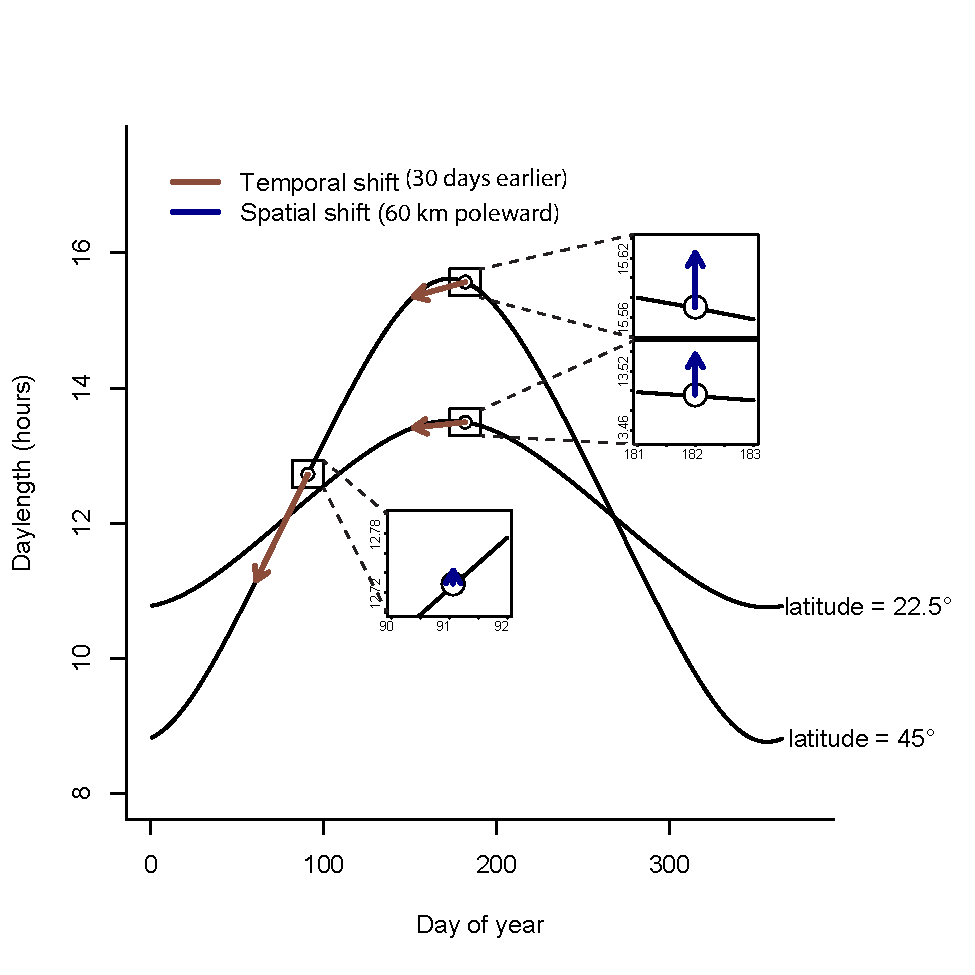
\includegraphics{..//..//analyses/photoperiod/figures/photo_spacetime_v2.pdf} %
\caption{\textbf{Photoperiod varies with latitude and by day of year}, such that temporal shifts in activity yield larger changes in experienced photoperiod compared with spatial shifts. Here, we show this variation at two latitudes (22.5\degree, 45\degree), using hypothetical spatial and temporal shifts. These shifts, based on observed average rates with recent global warming---16.9 kilometers per decade, or approximately 1.5 degrees in 100 years, for spatial shifts \citep{parmesan2006}, and 2.3 days per decade, or 23 days in 100 years, for temporal shifts \citep{chen2011})---highlight the greater magnitude in daylength changes close to the equinox (e.g., day of year 91), versus close to the summer solstice (e.g., day of year 182).}
 \label{fig:spacetime}%
 \end{figure}
 
 \begin{figure}[p]
\centering
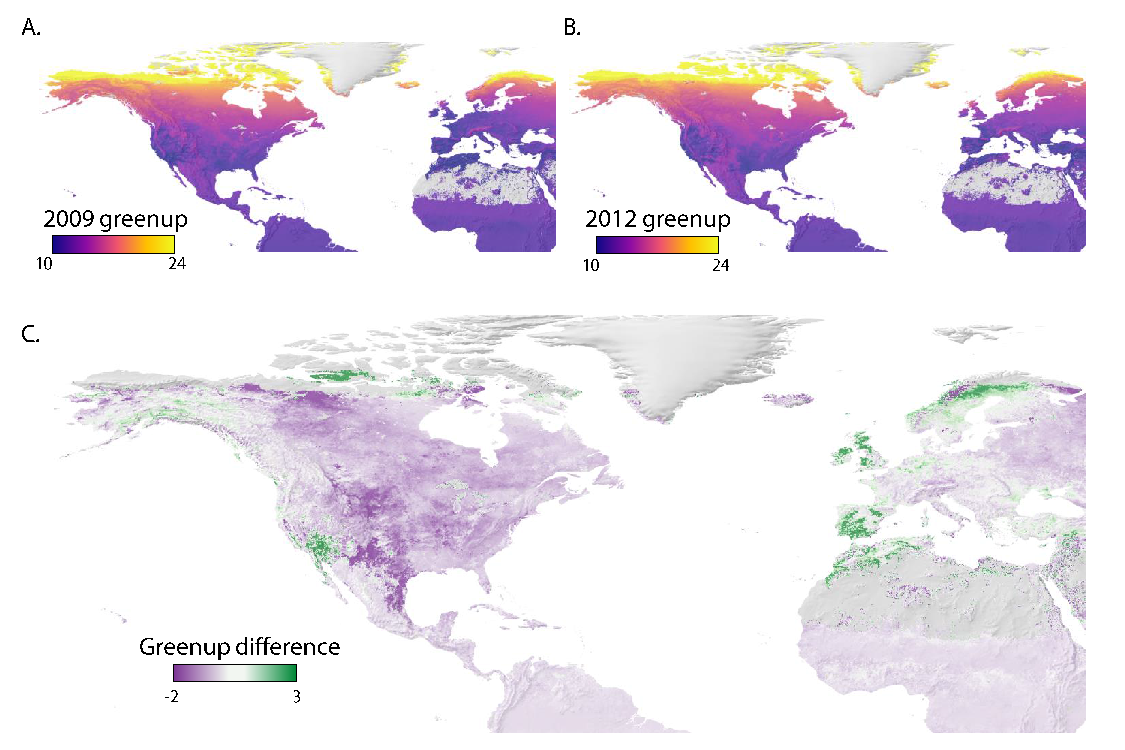
\includegraphics{..//..//docs/photoperiod/figures/Greenup_corr_lets.pdf} %2009 greenup
\caption{\textbf{Photoperiod on the ``green-up" date varies over space and between years} ``Green-up" is the beginning of seasonal greening, identified by satellite remote sensing measurements taken regularly throughout the year of the concentrations of green leaf vegetation. Hours of daylight on the date of spring green-up (here from MODIS satellite data) across North America and Europe for an average (2009, A) and  early (2012, B) North American start of spring. The differences between the years (in hours of daylength) are shown in (C). A negative difference signifies earlier green-up in 2012 versus 2009; a positive difference is the result of later green-up in 2012 compared with 2009. See `Quantifying and mapping differences in green-up across the United States and Europe' in the Supplemental Materials for more details. }%
 \label{fig:greenup}%
 \end{figure}
 
\begin{figure}[p]
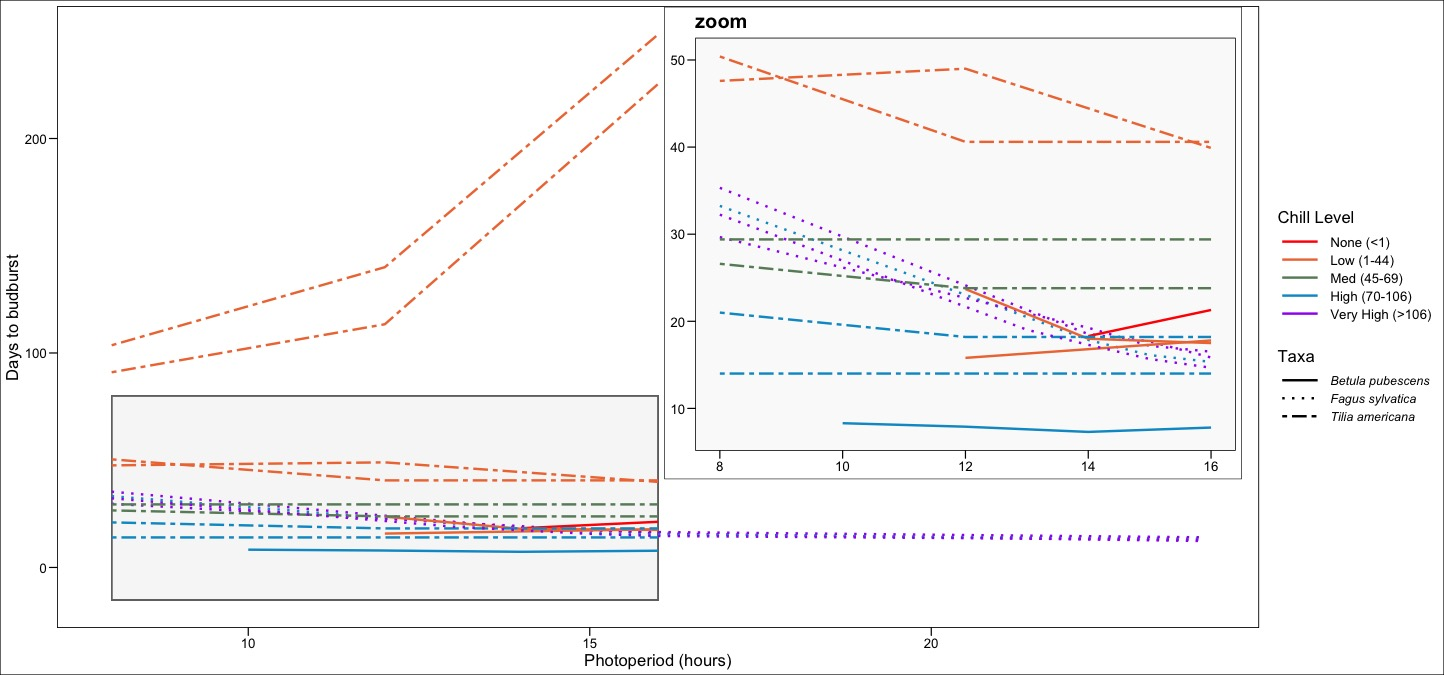
\includegraphics{..//..//analyses/photoperiod/figures/Photo_curv_FINAL.jpeg} 
\caption{\textbf{Nonlinearities in phenological responses to daylength} are apparent in spring woody plant phenology experiments (from the OSPREE database) in which three or more photoperiod treatment levels were applied. The shape of the response curves for \textit{Betula pubescens} \citep{Caffarra:2011b}, \textit{Fagus sylvatica} \citep{Heide:1993a} and \textit{Tilia americana} \citep{Ashby:1962aa} differ depending on the amount of winter chilling received (measured in Chill portions). Species and chilling levels with multiple lines represent plant material from different populations.}


 \label{fig:photocurve}
 \end{figure}


\begin{figure}[p]
\centering
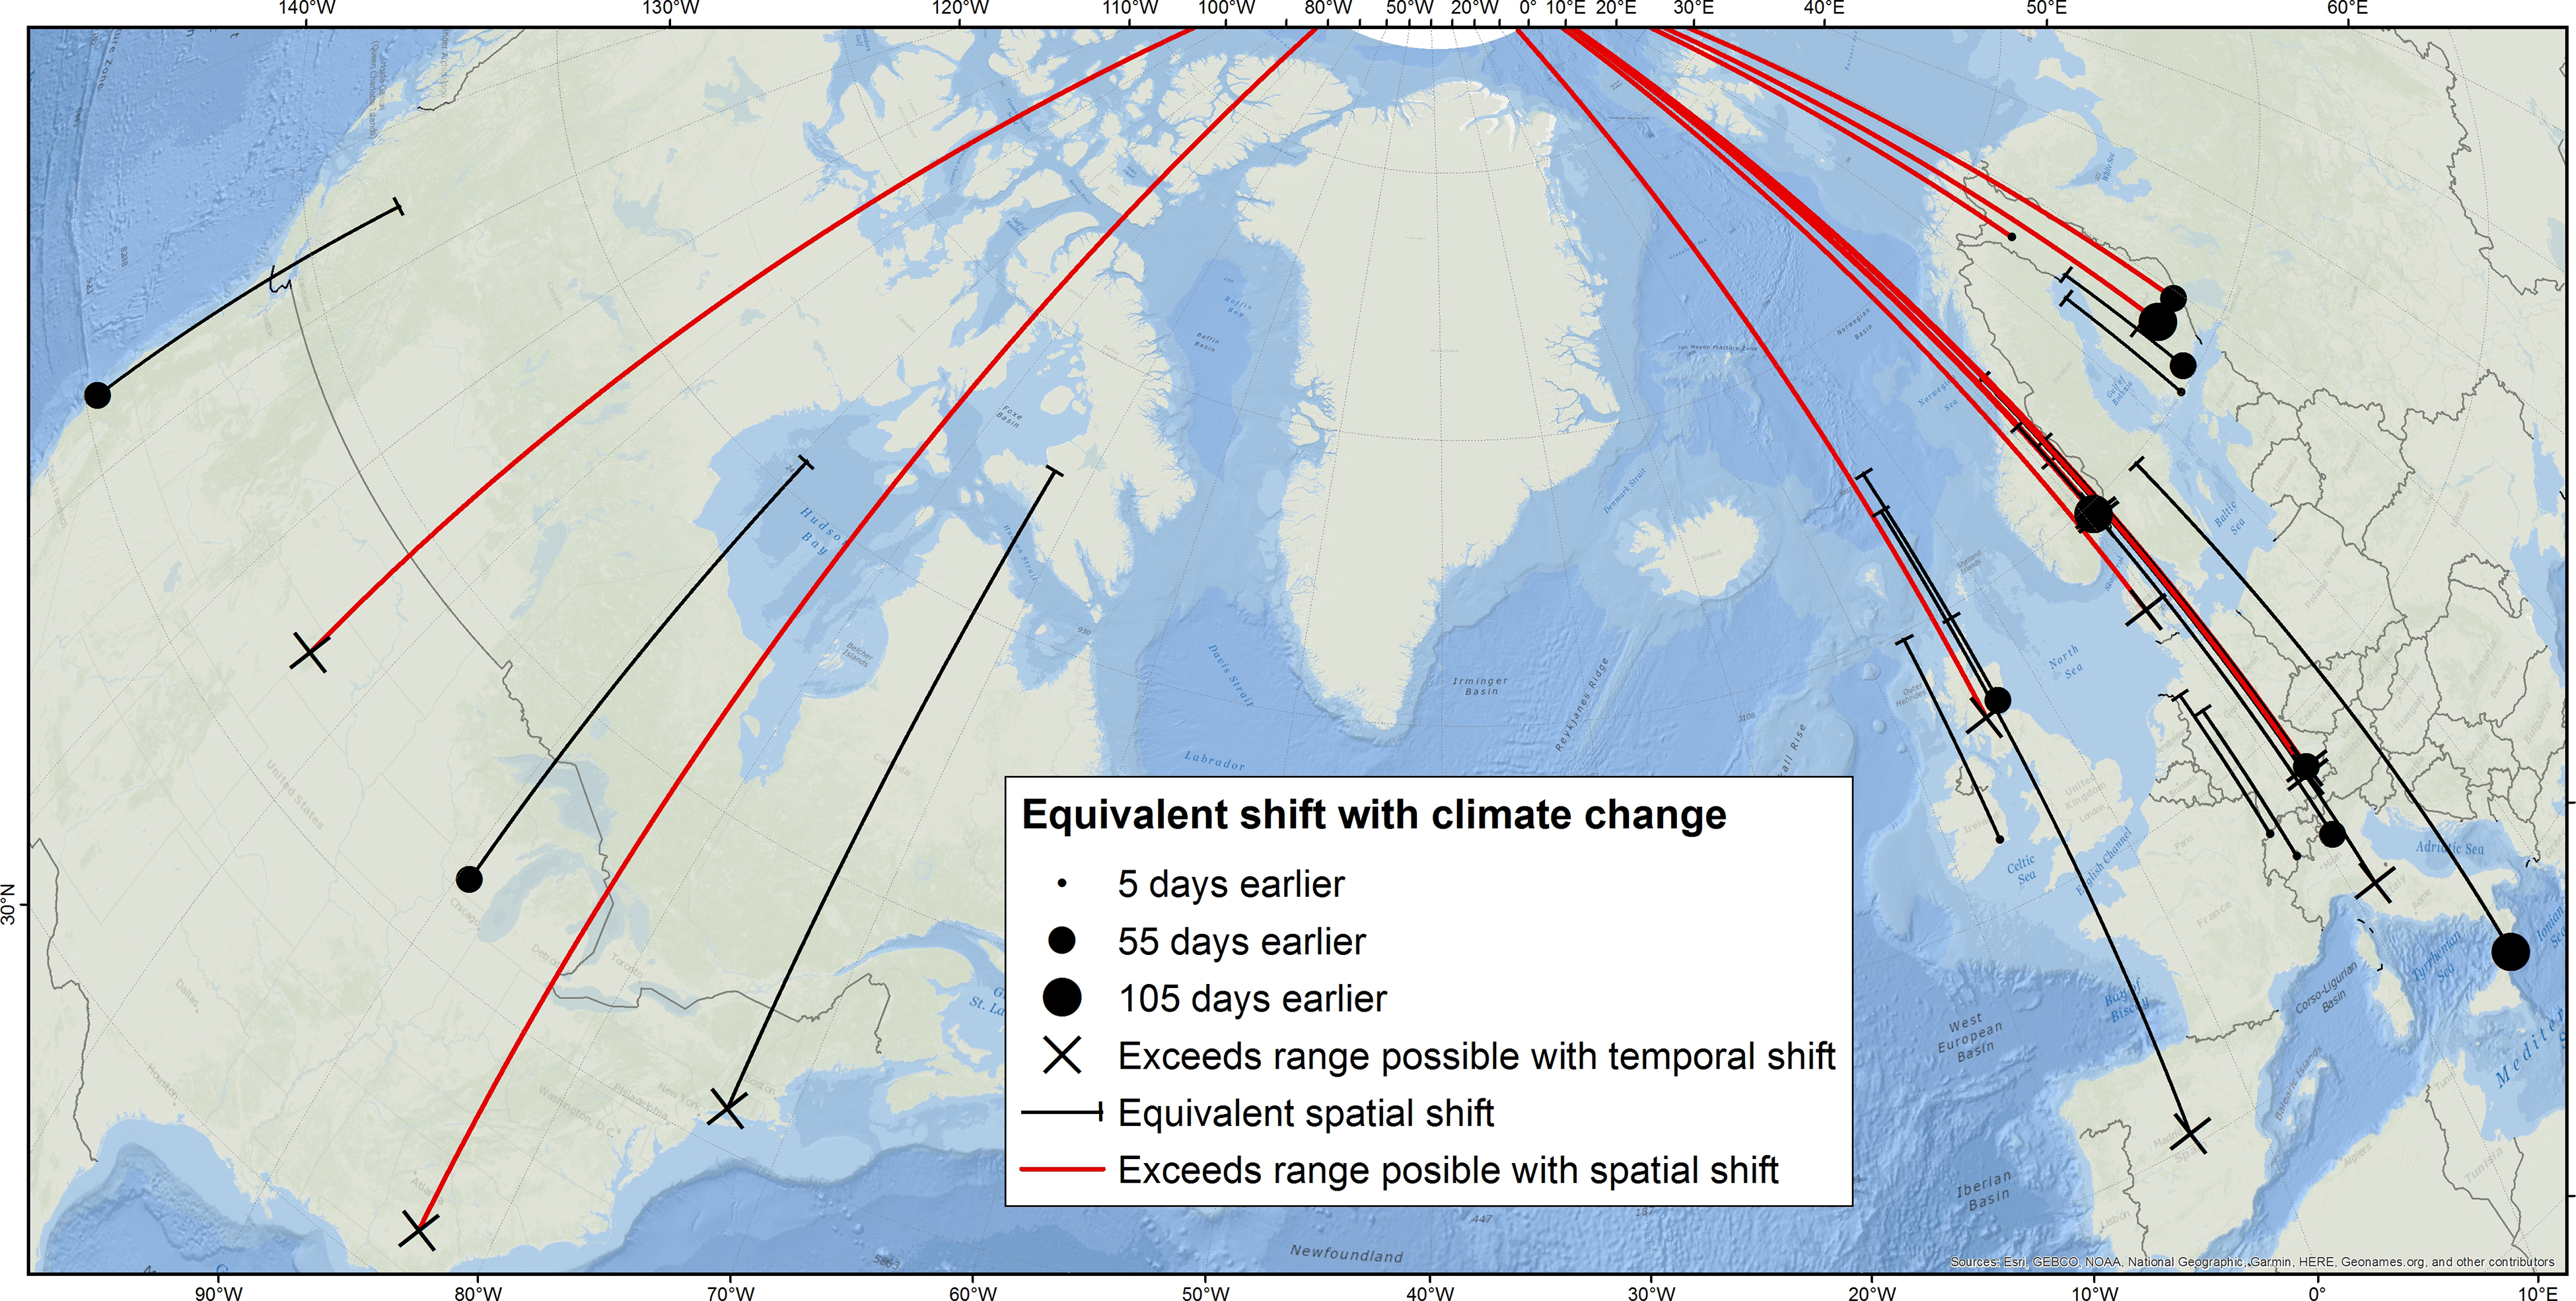
\includegraphics{..//..//analyses/photoperiod/figures/ospree_photopmap_fromblake.jpg} 
\caption{\textbf{Experimental photoperiod treatments and their equivalent spatial and temporal shifts} for experiments in the OSPREE database that manipulated photoperiod. See `Mapping temporal and spatial shifts in space and time' in the Supplemental Materials for details on how we calculated the required spatial (lines) or temporal (circles and Xes) shifts to be equivalent to photoperiod treatments in each experiment.}
 \label{fig:photomap}
 \end{figure}

 
\begin{figure}[p]
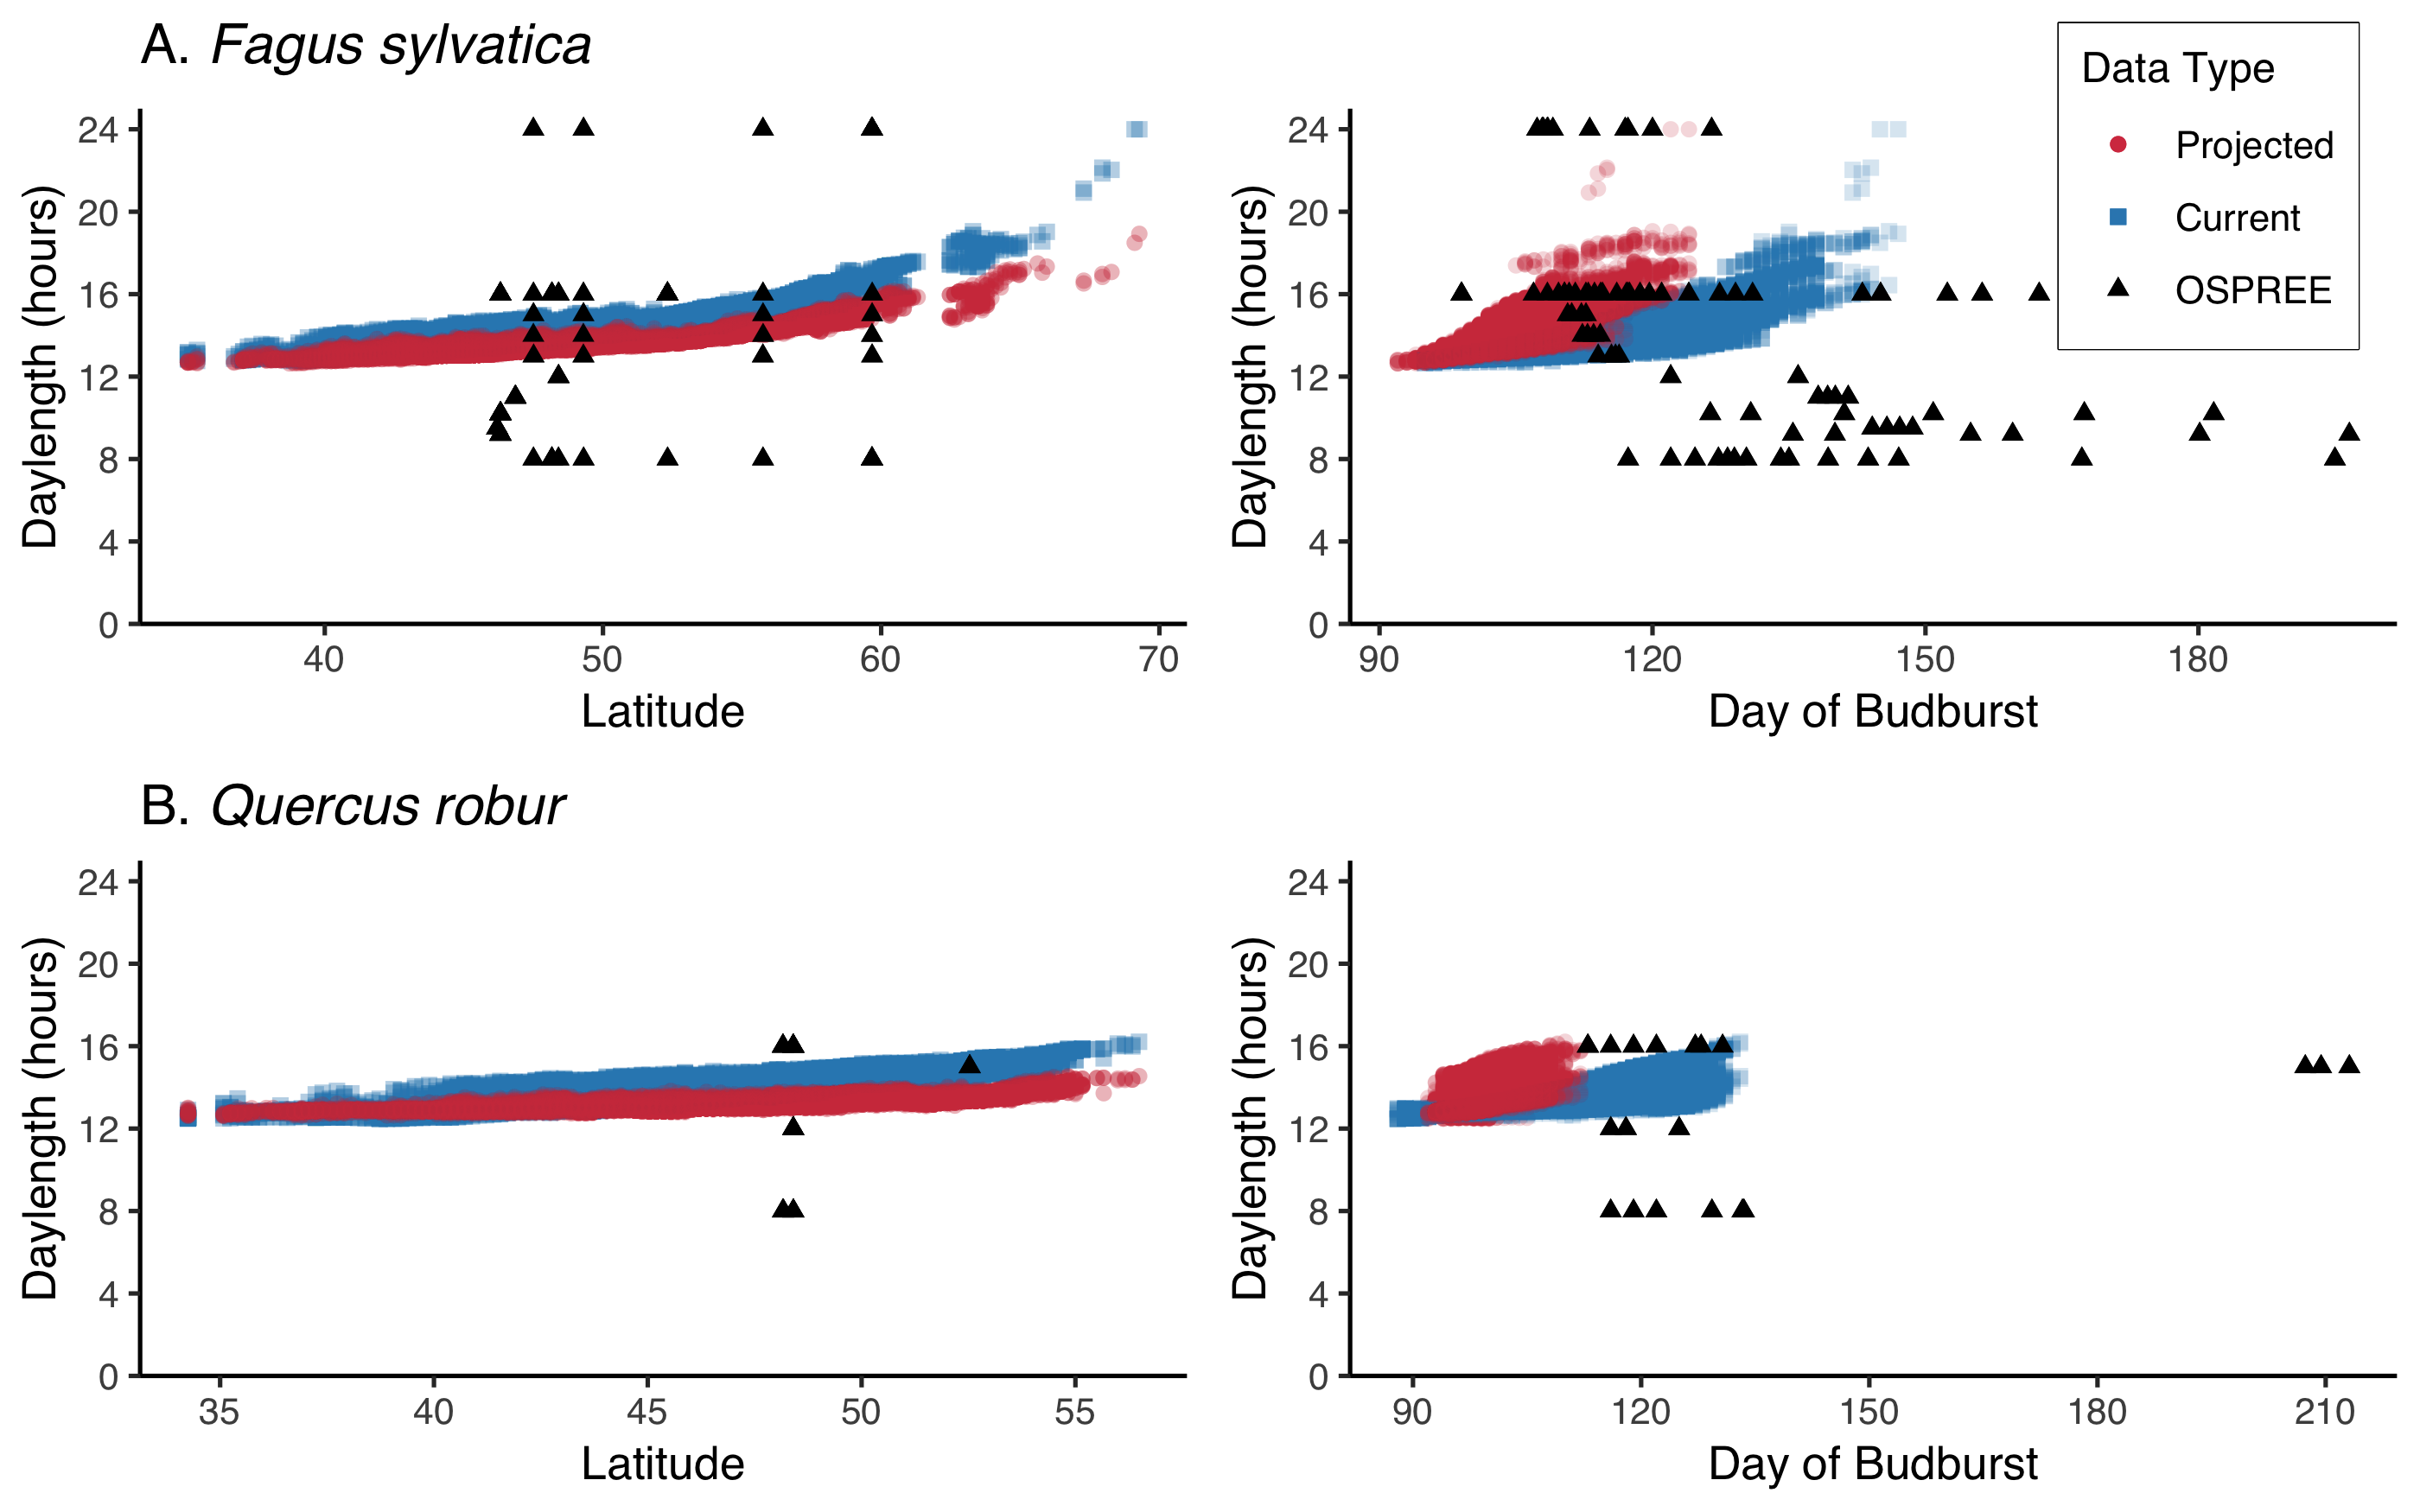
\includegraphics{..//..//analyses/photoperiod/figures/2D_actual_combined.png} 
\caption{\textbf{Experienced photoperiods in experiments differ from those in the natural world}, shown here by latitude (left panels) and by day of budburst (right panels) for \emph{Fagus sylvatica} (A, upper panels) and \emph{Quercus robur} (B, lower panels). Triangles show experimental treatments of photoperiod in the OSPREE database. To illuminate potential gaps between experiments and the natural world, we show the photoperiod when budburst occurs in its current (1981-2000) and projected ranges \citep[2081-2100, using the A1Fi Phenofit scenario, see][]{duputie2015}. We scaled the days to budburst for all OSPREE data points by adding the day of budburst from the first Phenofit observation. See Supplemental Materials and \citet{duputie2015} for additional details.} 
 \label{fig:fagus}
 \end{figure}
 
\begin{figure}[p]
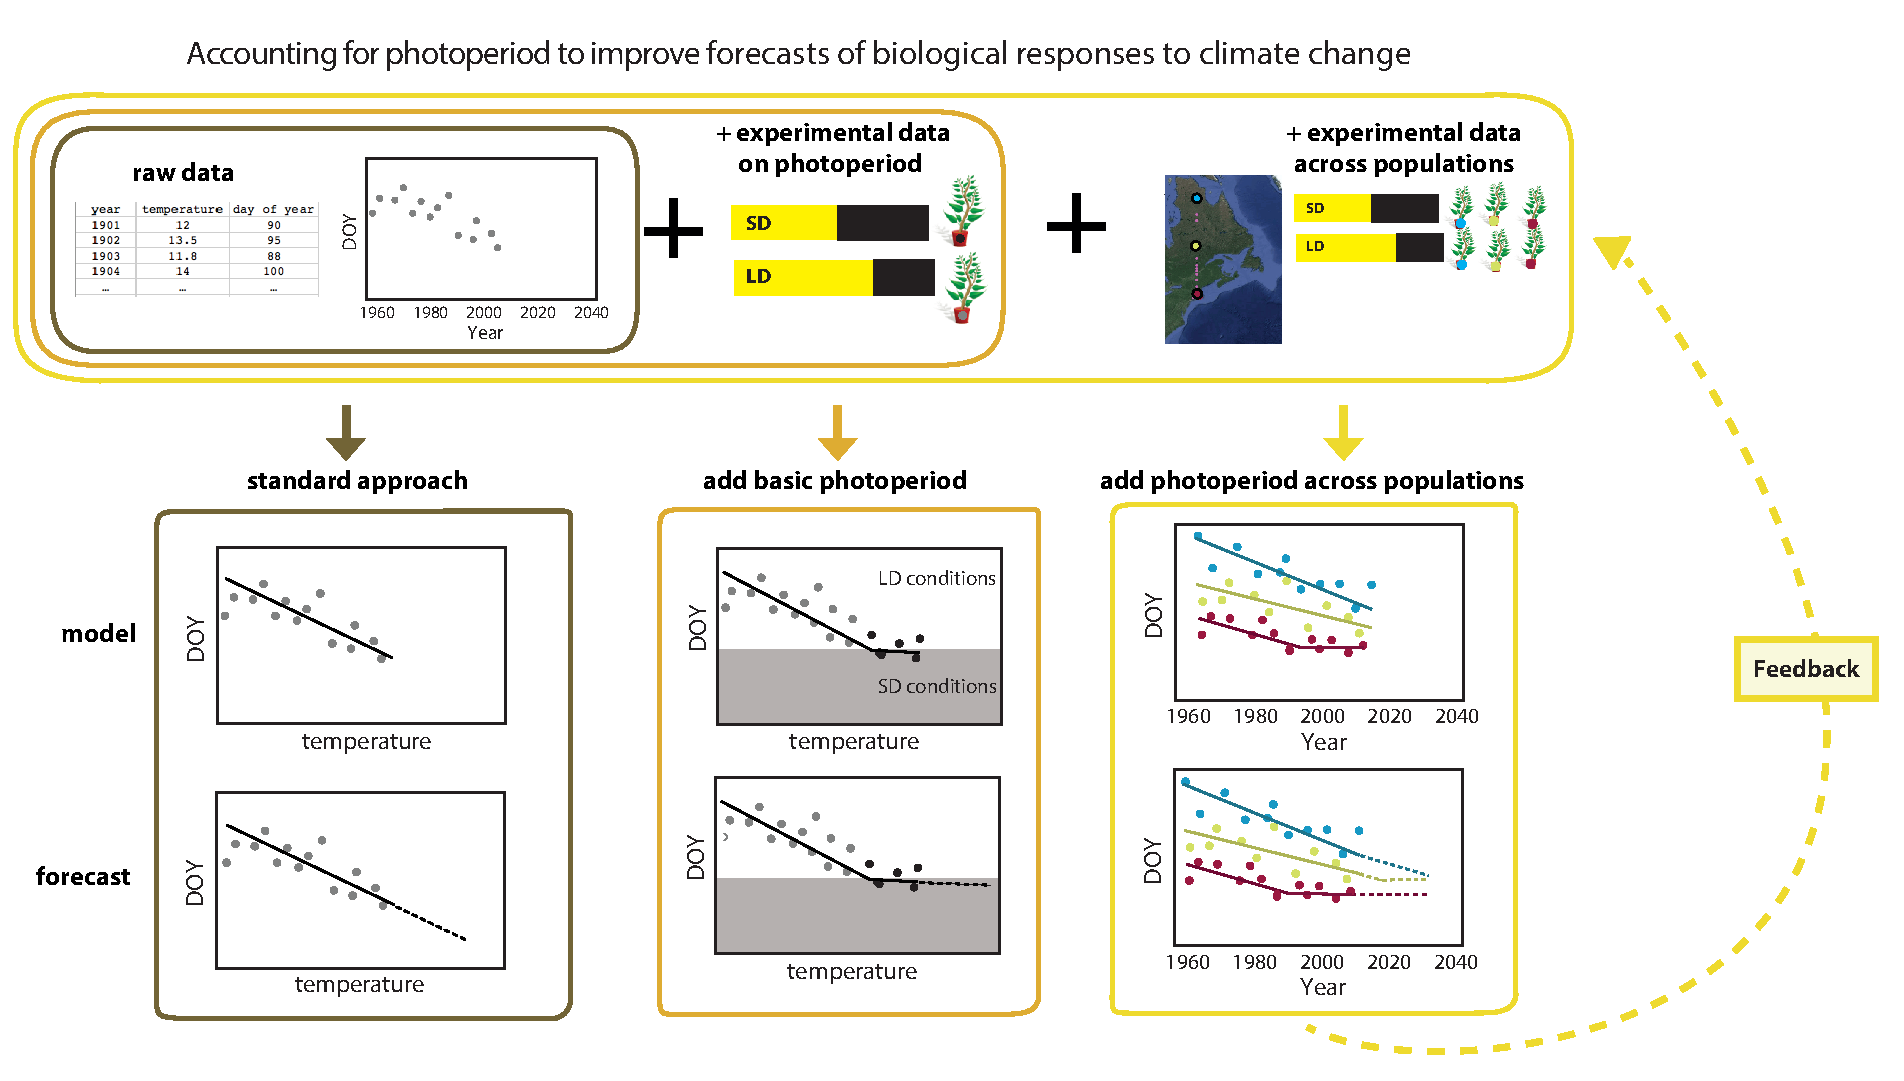
\includegraphics{..//..//analyses/photoperiod/figures/photocondiag6.pdf} 
\caption{\textbf{Conceptual diagram of how to include photoperiod in forecasting biological responses to climate change}. Current approaches for forecasting spring phenology with climate change frequently rely on linear relationships between historical temperature data and observed dates of spring phenology (left panels). Adding responses to photoperiod, which commonly operate as threshold responses to short days (SD) versus long days (LD, see ``photoperiod sensitivity" in the \emph{Glossary}), will alter these forecasts (center panel) in ways that differ across species with divergent threshold photoperiods. Other factors that interact with photoperiod, such as population-level variation in photoperiod responses, can be incorporated into forecasts to further improve their accuracy (right panel).}
 \label{fig:condiag}
 \end{figure}
 
 %Other examples of photoperiod control that could be used:
%1.  Onset  and  end  of post-juvenile  moult in migratory warblers and  the  onset  of  autumn  migratory  restlessness  are  advanced in short photoperiods. End  of autumn migratory restlessness, the onset and end of the winter moult  and  the  onset  of  spring  migratory  restlessness  are advanced  by  long  photoperiods. 

%2. temperature and photoperiod control of diapause induction in Lepidoptera https://academic.oup.com/ee/article-abstract/47/5/1314/5032483?redirectedFrom=fulltext

%3. An 1960s review of photoperiod and insect diapause https://www.jstor.org/stable/2459459?seq=1#metadata_info_tab_contents

%A model of a biocontrol insect that includes photoperiod and growing degree days https://www.fs.fed.us/foresthealth/technology/pdfs/BCIP_2013_Grevstad_Proposal.pdf

%%%%%%%%%%%%%%%%%%%%%%%%%%%%%%%%%%%%%%%%
\end{document}
%%%%%%%%%%%%%%%%%%%%%%%%%%%%%%%%%%%%%%%%
